\documentclass{article}
\usepackage{graphicx}
\usepackage{setspace}
\usepackage{amsmath}
\usepackage{kbordermatrix}
\usepackage{graphicx}
\graphicspath{{latex_pictures/}}
\doublespacing

\begin{document}

\title{}
 
\author{Jesse Zhang}
 

 
\maketitle % this produces the title block
 
\begin{abstract}
If you use this template and follow the instructions therein,
your will be able to write a paper using LaTeX.
\end{abstract}
 
\section{Purpose}

The purpose of the parser is to take a phylogenetic tree via variations of Newick notation, and create a distance matrix based on the taxa given via the Unrooted STAR method(U-STAR). The parser was written in R. 

\section{Concept}
Given the Newick notation $(((A,B),C),(D,E))$ we wish to obtain the distance matrix: \[
 \kbordermatrix{
	& A & B & C & D & E \\
	A & 0 & 2 & 3 & 4 & 4 \\
	B & 2 & 0 & 3 & 4 & 4 \\
	C & 3 & 3 & 0 & 3 & 3 \\
	D & 4 & 4 & 3 & 0 & 2 \\
	E & 4 & 4 & 3 & 2 & 0
}
\]

In order to achieve this we determine which taxon to resolve first and form named nodes to help condense the Newick notation until we have two or three remaining taxa/node names. Visualizing the following Newick notation via a distance tree gives the following, with each branch having a length of one. \newline
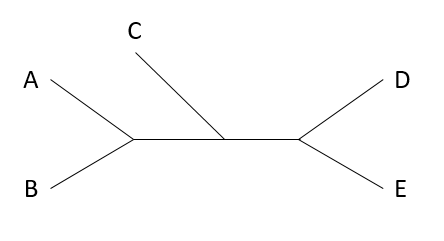
\includegraphics{firstTree.PNG}

Based on the given Newick notation we wish to resolve the innermost taxon first, this is done by finding priority, which produces a table such as the one seen below.

\begin{center}
	\begin{tabular}{ |c|c| } 
		\hline
		Taxon/Node Name & Priority  \\
		\hline
		 A & 3 \\ 
		 \hline
		 B & 3 \\ 
		 \hline
		 C & 2 \\
		 \hline 
		 D & 2 \\
		 \hline 
		 E & 2 \\ 
		\hline
	\end{tabular}
\end{center}

As soon in fig 3 we wish to resolve taxon A and B first, the resultant will be the creation of a named node with a distance vector from the taxa. This will reduce the tree removing A and B and instead replace both with a named node as seen below. \newline

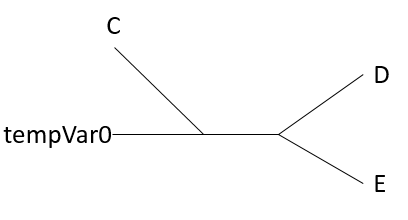
\includegraphics{secondTree.PNG} 

We also lower the named nodes priority by 1, it will also have the associated distance vector:
\[
\kbordermatrix{
	& \\
	A & 1 \\
	B & 1 \\
	C & 0 \\
	D & 0 \\
	E & 0
}
\]

The priorities 
\begin{center}
	\begin{tabular}{ |c|c| } 
		\hline
		Taxon/Node Name & Priority  \\
		\hline
		tempVar0 & 2 \\ 
		\hline
		C & 2 \\
		\hline 
		D & 2 \\
		\hline 
		E & 2 \\ 
		\hline
	\end{tabular}
\end{center}
\section{Methodology}
 
\subsection{Setup Phase:}

This parser is limited to binary trees in Newick notation but allows for trees to be unrooted or rooted, with or without metric information.

When first given Newick notation, it will first remove all numeric data, leaving only the topological form of the tree. In order to remove numeric data, we pass through the input twice first removing branch lengths, related symbols, and extraneous whitespace. An example of this is given the Newick form $((AN3C:.1,B1ED:.2)123:.15,(CAS2:.1,DE4D:.05 )125:.2)$ it will be reduced to $((AN3C,B1ED),(CAS2,DE4D))$. 

Upon successfully simplifying the Newick notation, we extract all the taxa names as delimited by parentheses and commas they are then store them as a 1 by $X$ character array where $X$ is the number of taxa. The variable used to store these taxa is called {\tt myVars} and will be referenced multiple times through the program. 

After finding the taxa names we will initalize a list of lists called {\tt matrixList} with length $X$. Each {\tt matrixList} index has three parts, a taxon name({\tt var}), its priority({\tt value}) which is set to zero, and a 1 by $X$ vector({\tt varMatrix}). The 1 by $X$ vector will have its entries indexed by the taxon names with each initial entry being stored as a zero. {\tt value} slot will be used to decide what taxon to process first in the {\tt matrixList}.

After initialization of the {\tt matrixList} we will then determine priority for each taxon. We remove taxon names from the Newick notation temporarily replacing them white whitespace. For example $((A,B),C)$ becomes $((\_,\_),\_)$ this will allow us to ignore the taxa names in order to establish priority. We will read through this character by character. We initialize two variables that will be modified throughout, priority which is set to zero and count, which is set to one. If the char is a left parenthesis we increment the priority by one, if the char is a right parenthesis we decrease the priority by one. Finally, if the char is a whitespace we will store priority in the appropriate count index in matrixList and increment count by one. Note, as myVars/matrixList was initialized from left to right, the first whitespace on the left corresponds to the first matrixList index, the second whitespace corresponds to the second matrixList index, and a similar pattern for the remaining whitespaces. The result is a matrixList populated with their associated priority. 

The final distance matrix is initialized at this point as a $X$ by $X$ matrix. We will then set the column names and row names to the associated taxa names store in {\tt myVars}. 

\subsection{Algorithm}

Setting priority is important as we wish to compute the innermost taxa first For example in $((A,B),C)$. We would need to resolve A and B in a distance matrix before finally resolving it with taxa C. The program is set to be in a while loop to continue while the length of the matrixList is greater than two. In the while loop we will sort the variables by its priority and then make note of the highest priority variables in an indexList, which is preallocated with a default size of 100.

Within the while loop after properly indexing the highest priority of matrixList we enter a for loop that resolves two indexes of matrixList at a time. Within the algorithm there exists two classifications of indexes of matrixList, an index with a distance matrix and an index with an empty matrix. This leads to three cases after looking at both variables, if there are only two taxas then the finalMatrix will enter the values of having a distance two apart, it will then delete both entries and replace it with a temporary variable, and populate a distance matrix with a distance of one from each of the two original taxa. The R code is setup to generate any temporary variable to start with tempvar0, temvar1, etc… The value of this is then reduced by one thus lowering its priority. 

In the case of one taxa and one matrix it will iterate through the matrix and for each value greater than zero it will enter it to the corresponding finalMatrix with the taxa giving it the value in the matrix plus additional two for the total branch length. Afterwards a temporary variable will be created with the current non-zero values in the matrix being incremented by one with the taxa being added afterwards with a value of one.

In the case of two matrixes we will utilize a nested for loop, for each non-zero value in the first matrix it will iterate the second matrix and find non-zero values. Once the second non-zero value is acquired the appropriate slot in the finalMatrix will be filled with the first value plus the second value plus an additional two for branch length. Afterwards we will develop a temporary variable by combining the two matrix values and incrementing each value greater than zero by one.

Similar cases proceed for the last two variables however branch lengths are treated differently. Follow these above cases but instead entries into the finalMatrix are one less. The other case is with three final taxa/matrix groupings. 

Within the four cases if all are taxa we will set a distance of two between all variables and enter it in the distance matrix. In the case of one matrix in two remaining taxa we will identify the index of the matrix and then enter it with the other two taxa for non-zero values plus two into the finalMatrix. Finally the last two taxa will be entered with a length of two apart. For two matrixes one taxa we use a similar example to how two matrix’s normally resolve and create a temporary matrix to then enter the finalMatrix values with the taxa. For three matrix it follows a similar step for two matrix but resolves the temporary matrix with the final matrix. 


\end{document}


